\documentclass[10pt,twocolumn]{article}

\usepackage[a4paper,margin=18mm]{geometry}
\usepackage[T1]{fontenc}
\usepackage{times}
\usepackage{microtype}
\usepackage{amsmath,amssymb}
\usepackage{graphicx}
\usepackage{booktabs}
\usepackage{array}
\usepackage{tabularx}
\usepackage{xcolor}
\usepackage[hidelinks]{hyperref}
\usepackage{enumitem}
\usepackage{float}
\usepackage{tikz}
\usetikzlibrary{arrows.meta,positioning}

\setlength{\textfloatsep}{8pt plus 1pt minus 2pt}
\setlength{\dbltextfloatsep}{8pt plus 1pt minus 2pt}
\setlength{\floatsep}{8pt plus 1pt minus 2pt}
\setlength{\intextsep}{8pt plus 1pt minus 2pt}

\title{\vspace{-6mm}\textbf{From Forecasts to Realized Decisions: Why Forecast-to-Execution Interfaces Matter Under Frictions}\vspace{-2mm}}
\author{}
\date{}

\begin{document}

\twocolumn[{%
\maketitle
\vspace{-6mm}
\begin{abstract}
Forecasting-driven decision systems are often assessed as if proposed targets were immediately realized. Under frictions, proposed targets and realized actions can diverge, so prediction-side metrics alone can misstate realized system quality. We study a forecast-to-execution interface that separates proposed targets from realized executed decisions and attaches primary evaluation to the executed path while holding predictive information fixed. In a narrow cost-sensitive portfolio case study with a frozen learned policy, the validation-selected interior operating point $\eta=0.5$ improves held-out executed-path net Sharpe relative to $\eta=1.0$ in positive-cost regimes while roughly halving executed turnover, and the zero-cost row remains near-flat. Accounting diagnostics and conservative supporting analyses support the same conclusion: this is an implementation-side evaluation result rather than evidence of a stronger predictor.
\end{abstract}
\vspace{1mm}
\hrule
\vspace{2mm}
}]

\section{Introduction}

Forecasting-driven systems are often evaluated at the level of proposed outputs, as if those outputs were directly realized by downstream decision layers. Under frictions or implementation constraints, however, proposed targets need not coincide with realized actions. This creates an evaluation problem: forecast quality and realized decision quality are not the same object once a forecast-to-decision interface intervenes. The central question is therefore not only whether forecasts look good before implementation, but also whether the system is evaluated on the realized path it actually induces.

We study this general evaluation issue in a concrete cost-sensitive portfolio case study. The portfolio setting is the evidence source rather than the paper's identity: predictive information is held fixed, target-level quantities remain diagnostic only, and primary evaluation is attached to executed-path outcomes as the forecast-to-execution interface is varied. In the central selected-point comparison, the validation-selected interior operating point $\eta=0.5$ is evaluated against the immediate-execution baseline $\eta=1.0$; the positive-cost rows improve, while the zero-cost row remains near-flat. The contribution is therefore an implementation-side evaluation argument for forecasting-driven decision systems, not a stronger-prediction claim and not a new RL-method claim.

The paper makes three narrow contributions. First, it frames forecast-to-decision evaluation around the distinction between proposed targets and realized actions under frictions, and argues that executed-path evaluation should be primary while target-level quantities remain diagnostic. Second, it provides fixed-signal evidence from a cost-sensitive portfolio case study showing that the validation-selected interior operating point $\eta=0.5$ improves positive-cost held-out executed-path performance relative to $\eta=1.0$, while the zero-cost row remains near-flat. Third, it provides supporting evidence from accounting diagnostics and a conservative same-forecast analysis showing that forecast-side movement can stay small even when realized decision-side consequences become large.

\section{Forecast-to-Execution Interface}

Figure~\ref{fig:conceptual} gives the paper's core framing. Forecast outputs first become proposed targets and only later become realized actions after passing through an execution interface. Once frictions or implementation constraints intervene, the proposed target is no longer the same object as the realized decision. That distinction matters because the system is ultimately experienced through realized trading, realized cost, and realized decision quality rather than through the counterfactual target alone.

The interface perspective changes the evaluation question. The issue is not whether target-level quantities are meaningless; they remain useful diagnostics. The issue is that they answer a different question from the one the deployed decision system actually faces. For that reason, this workshop paper treats the executed path as the primary evaluation object and uses target-level summaries only to explain where target and realized paths diverge.

\begin{figure*}[t]
\centering
\resizebox{0.97\textwidth}{!}{%
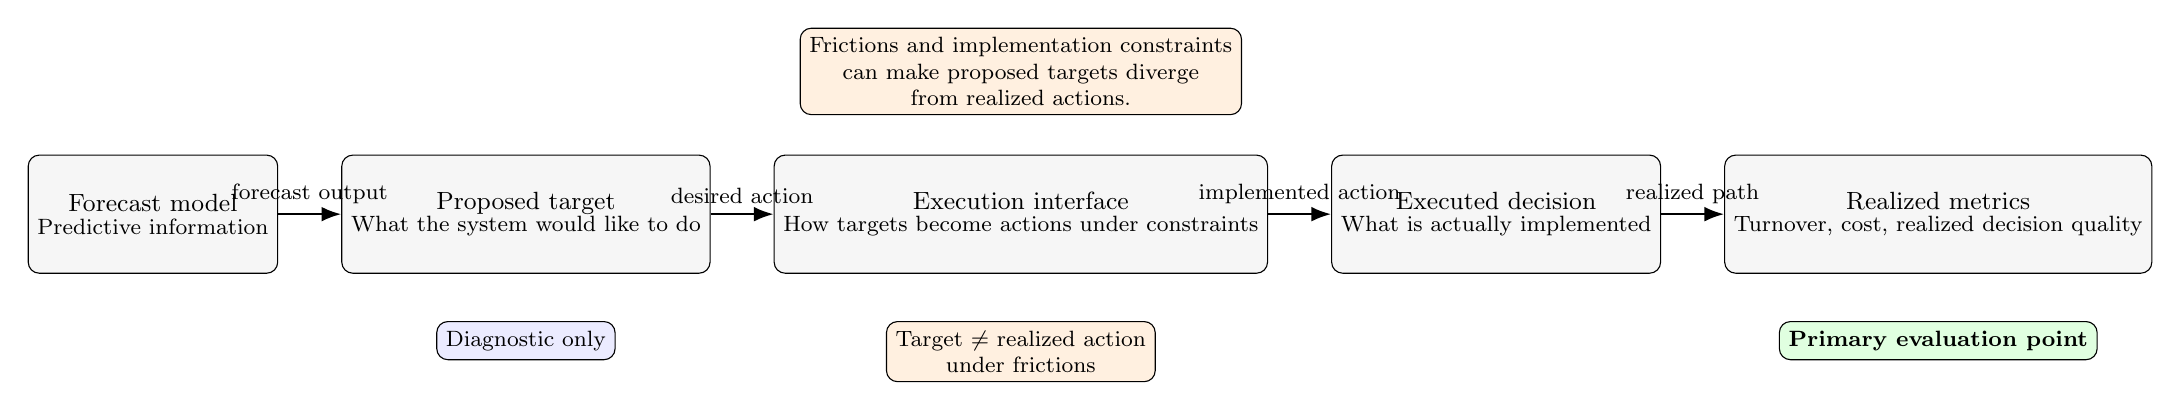
\begin{tikzpicture}[
  node distance=8mm,
  box/.style={draw, rounded corners, minimum width=2.45cm, minimum height=1.5cm, align=center, font=\small, fill=gray!7},
  note/.style={draw, rounded corners, align=center, font=\footnotesize, fill=orange!12},
  eval/.style={draw, rounded corners, align=center, font=\footnotesize\bfseries, fill=green!12},
  arr/.style={-{Latex[length=2.5mm]}, thick}
]
\node[box] (forecast) {Forecast model\\[-1mm]\footnotesize Predictive information};
\node[box, right=8mm of forecast] (target) {Proposed target\\[-1mm]\footnotesize What the system would like to do};
\node[box, right=8mm of target] (iface) {Execution interface\\[-1mm]\footnotesize How targets become actions under constraints};
\node[box, right=8mm of iface] (exec) {Executed decision\\[-1mm]\footnotesize What is actually implemented};
\node[box, right=8mm of exec] (metrics) {Realized metrics\\[-1mm]\footnotesize Turnover, cost, realized decision quality};

\draw[arr] (forecast) -- node[above, font=\footnotesize] {forecast output} (target);
\draw[arr] (target) -- node[above, font=\footnotesize] {desired action} (iface);
\draw[arr] (iface) -- node[above, font=\footnotesize] {implemented action} (exec);
\draw[arr] (exec) -- node[above, font=\footnotesize] {realized path} (metrics);

\node[note, above=5mm of iface] (friction) {Frictions and implementation constraints\\can make proposed targets diverge\\from realized actions.};
\node[note, below=6mm of iface] (gap) {Target $\neq$ realized action\\under frictions};
\node[eval, below=6mm of metrics] (evalpoint) {Primary evaluation point};
\node[note, below=6mm of target, fill=blue!8] (diag) {Diagnostic only};
\end{tikzpicture}
}
\caption{From forecasts to realized decisions under frictions. The conceptual diagram shows how predictive outputs become proposed targets and then realized actions once a forecast-to-execution interface and frictions intervene. Its role is to make the workshop framing explicit: forecast quality and realized decision quality are related but not identical, so evaluation should follow realized actions rather than targets alone.}
\label{fig:conceptual}
\end{figure*}

\section{Experimental Setup}

The empirical setting is intentionally narrow. We use a fixed 27-name portfolio snapshot under the canonical frozen split and hold the learned policy and predictive information fixed across execution arms. The main comparison is therefore not a retraining study. Instead, it isolates how realized outcomes change when only the forecast-to-execution interface is varied.

The selected-point protocol compares the validation-selected interior operating point $\eta=0.5$ against the immediate-execution baseline $\eta=1.0$ on the main cost rows $\kappa\in\{0, 5\times10^{-4}, 10^{-3}\}$. The primary metric is executed-path net Sharpe. Executed turnover is reported as supporting evidence because the mechanism of improvement is expected to operate through realized trading intensity and realized cost. This setup keeps the paper focused on one identification question: whether changing only the forecast-to-execution interface changes realized decision quality under frictions.

\section{Results}

The first empirical question is evaluative rather than domain-specific: once frictions separate proposed targets from realized actions, does changing only the forecast-to-execution interface change realized system quality? Table~\ref{tab:rl-main} answers that question in the paper's concrete portfolio case study. With the learned policy and predictive information held fixed, the validation-selected interior point $\eta=0.5$ improves held-out executed-path net Sharpe relative to the immediate-execution baseline $\eta=1.0$ by $+0.0105$ at $\kappa=5\times10^{-4}$ and $+0.0213$ at $\kappa=10^{-3}$, while reducing median executed turnover from $0.02200$ to $0.01095$. The $\kappa=0$ row remains near-flat at $-0.0002$, which is the expected zero-cost pattern under the documented interpretation. This is therefore best read as an implementation-side result that appears under frictions rather than as evidence of a stronger predictor.

\begin{table}[t]
\centering
\small
\resizebox{\columnwidth}{!}{\begin{tabular}{lrrrrr}
\hline
$\kappa$ & Net Sharpe ($\eta=1.0$) & Net Sharpe ($\eta=0.5$) & Paired-median $\Delta$ Sharpe & TOexec ($\eta=1.0$) & TOexec ($\eta=0.5$) \\
\hline
$0$ & 1.1542 & 1.1554 & -0.0002 & 0.02200 & 0.01095 \\
$5\times10^{-4}$ & 1.1340 & 1.1447 & \textbf{+0.0105} & 0.02200 & 0.01095 \\
$10^{-3}$ & 1.1127 & 1.1340 & \textbf{+0.0213} & 0.02200 & 0.01095 \\
\hline
\end{tabular}
}
\caption{Held-out executed-path comparison for the frozen-policy selected operating point. With predictive information held fixed, the validation-selected interior point $\eta=0.5$ is compared against the immediate-execution baseline $\eta=1.0$ on $\kappa\in\{0, 5\times10^{-4}, 10^{-3}\}$, showing positive-cost gains with a large reduction in executed turnover while the zero-cost row remains near-flat. The paired-median delta is computed on aligned seed-level outcomes and therefore need not equal the arithmetic difference between the displayed marginal medians. This is the paper's only main empirical result, because it isolates how the forecast-to-execution interface changes realized decision quality under frictions.}
\label{tab:rl-main}
\end{table}

Figure~\ref{fig:accounting} explains why executed-path evaluation is primary. Target-level quantities are diagnostic, not headline evaluation objects. At the validation-selected operating point $\eta=0.5$, target turnover is about twice realized executed turnover across the main cost rows, while tracking remains small but nonzero and the final path gap widens with cost. These diagnostics matter because proposed targets and realized positions are not the same object once frictions intervene. A narrow target-versus-executed evaluation comparison reaches the same conclusion more directly: in the positive-cost rows, executed-path evaluation favors $\eta=0.5$, while target-based evaluation is approximately flat to slightly negative. In other words, the choice of evaluation object is not merely presentational: in the positive-cost rows, target-based evaluation weakens or erases the selected-point improvement that remains visible on the realized executed path. The accounting package therefore explains the evaluation object used in the main result rather than competing with it.

A denser cost sweep in the appendix preserves the same friction-sensitive direction: the zero-cost row remains near-flat, while the realized executed-path advantage becomes more visible in the positive-cost rows.

The point is not that smoothing is intrinsically beneficial; rather, once frictions separate desired targets from realized actions, the forecast-to-execution interface becomes part of the evaluated system, and its effects must be assessed on the realized path.

\begin{figure}[t]
\centering
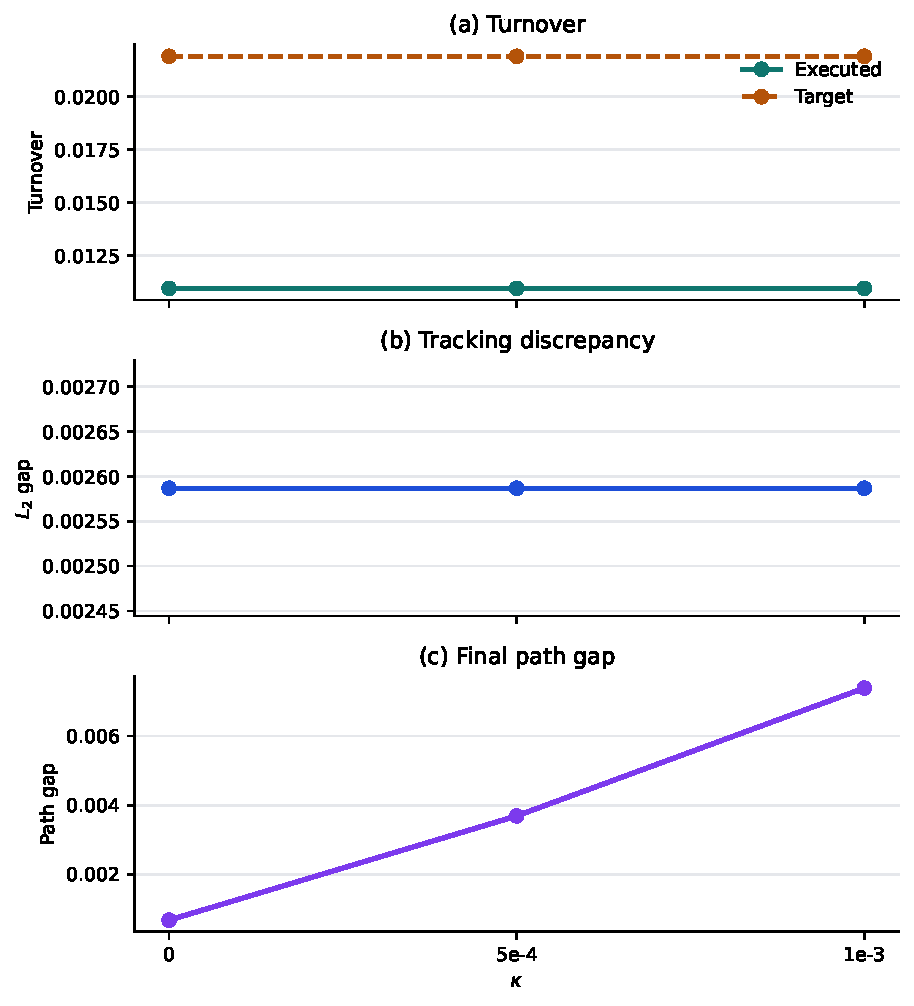
\includegraphics[width=\columnwidth]{assets/figures/fig_accounting_gap.pdf}
\caption{Why target-level evaluation can misstate realized decision quality. Diagnostic accounting summaries compare target-level and executed-path quantities at the validation-selected operating point $\eta=0.5$. Target turnover remains about twice executed turnover, tracking is small but nonzero, and the final path gap widens with cost, showing why the realized executed path rather than the target path is the primary evaluation object in this paper.}
\label{fig:accounting}
\end{figure}

A conservative supporting analysis, reported in the appendix under the title \emph{Similar forecasting information, different realized decision quality}, shows that forecast-side metrics move only slightly while decision-side metrics move much more strongly in the positive-cost rows. At $\kappa=5\times10^{-4}$ and $\kappa=10^{-3}$, forecast MSE shifts by only $-0.03\%$ and $+0.28\%$, whereas executed turnover and realized cost fall by $90.8\%$ and $95.1\%$, with net Sharpe rising by $+0.9539$ and $+2.0208$. This pattern is consistent with an interface-side interpretation, but because only metric-level similarity is established rather than raw forecast-vector identity, it remains appendix support rather than a main-text finding.

Additional materials should be referenced briefly and moved out of the core story. The appendix includes a denser cost-grid support figure and an auxiliary same-state CC-TA-LBIP comparator. Both move in the same qualitative direction as the main result, but neither should displace the selected-point comparison as the central empirical finding.

\section{Discussion and Limitations}

This workshop paper makes one narrow point: when frictions separate proposed targets from realized actions, forecasting systems should be evaluated on the realized path they actually induce. In our case study, the selected-point result and the accounting diagnostic support the same interpretation. Holding predictive information fixed, changing the forecast-to-execution interface changes realized turnover, realized cost, and realized decision quality. That is the paper's contribution, and it is best read as an evaluation result about forecasting-to-decision systems under frictions.

The first limitation is scope. This is a narrow portfolio-domain case study built on a fixed 27-name snapshot under the canonical frozen split rather than a broad cross-universe study. The evidence is informative because it isolates the forecast-to-execution interface while keeping the predictive signal fixed, but it is still drawn from one application setting. The paper therefore supports a concrete forecasting-to-decision evaluation argument rather than a universality claim.

The second limitation is the learning setup. The central identification result is a frozen-policy comparison rather than an end-to-end retraining study. That is useful for the workshop question because it keeps predictive information fixed, but it also means the evidence is about how realized decision quality changes under a different interface, not about how a jointly retrained system would behave. The remaining materials should stay in supporting roles: the denser cost-grid figure is appendix support, the CC-TA-LBIP package remains auxiliary same-state evidence, and the \emph{Similar forecasting information, different realized decision quality} table should remain conservative because exact forecast identity across arms has not been directly established. A denser cost-grid check strengthens the paper's friction-sensitive evaluation reading, but we do not elevate temporal robustness beyond the documented canonical split in this workshop version.

These limitations do not weaken the core reading; they locate it. The forecasting relevance of the paper is that it distinguishes forecast quality from realized decision quality in settings where forecasts pass through downstream implementation layers before becoming realized actions. A natural next step is to test the same evaluation logic in additional forecasting-driven domains, but the workshop contribution already stands on the narrower point established here: under frictions, evaluation should follow realized actions rather than targets alone.

\section{Conclusion}

This paper argues for a simple but important evaluation principle for forecasting-driven decision systems under frictions: realized actions, not proposed targets alone, should anchor primary evaluation. In the concrete portfolio case study here, the validation-selected interior execution interface improves positive-cost held-out realized performance while the zero-cost row remains near-flat, and a denser appendix cost sweep preserves the same friction-sensitive direction. More broadly, the same evaluation issue can arise whenever forecasting outputs pass through constrained implementation layers before they become realized actions.

\clearpage
\appendix
\setcounter{figure}{0}
\setcounter{table}{0}
\renewcommand{\thefigure}{A\arabic{figure}}
\renewcommand{\thetable}{A\arabic{table}}
\renewcommand{\theHfigure}{A\arabic{figure}}
\renewcommand{\theHtable}{A\arabic{table}}

\noindent\textbf{A. Denser Cost-Grid Support for the Friction-Sensitive Evaluation Pattern.}
The appendix cost sweep keeps the same evaluation-object reading on a denser six-point grid.
\par\medskip
\begin{figure}[H]
\centering
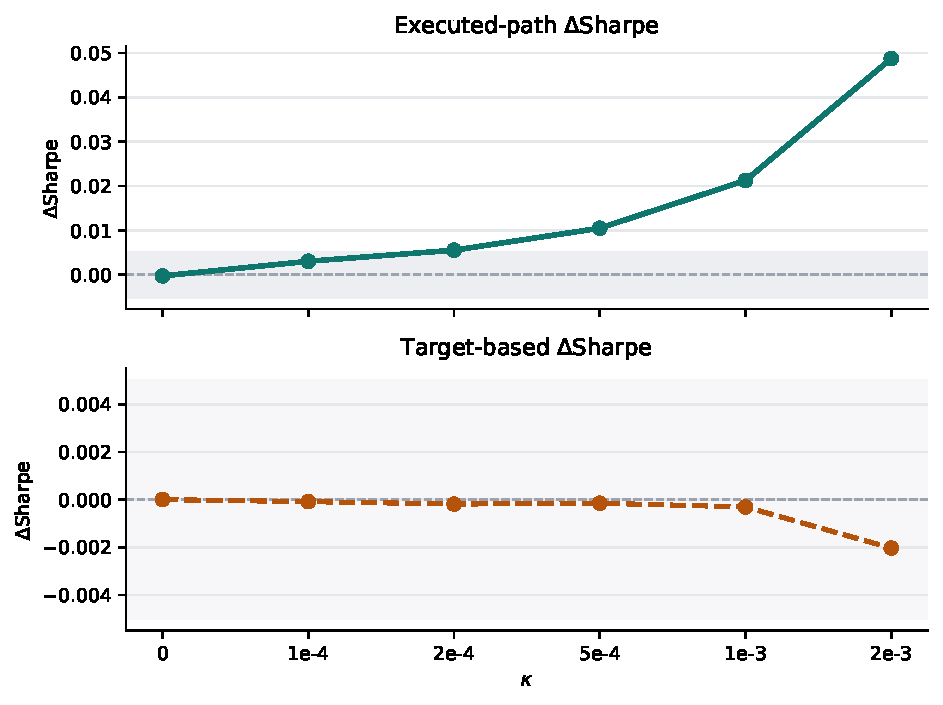
\includegraphics[width=\columnwidth]{assets/figures/fig_cost_sweep_appendix.pdf}
\caption{Denser cost-grid support for the friction-sensitive evaluation pattern. The executed-path delta remains near-flat at $\kappa=0$ and becomes more visible across positive-cost rows, while the target-based delta remains approximately zero or negative. This is appendix support for the paper's evaluation-object reading, not a new main result class.}
\label{fig:cost-sweep-support}
\end{figure}

\noindent\textbf{B. CC-TA-LBIP Auxiliary Evidence.}
\par\smallskip
\begin{table}[H]
\centering
\scriptsize
\resizebox{\columnwidth}{!}{\begin{tabular}{lrrrrrr}
\hline
$\kappa$ & selected $c$ & Net Sharpe ($c=0$) & Net Sharpe ($c=3000$) & $\Delta$ Sharpe & TOexec ($c=0$) & TOexec ($c=3000$) \\
\hline
$0$ & 3000 & 1.1875 & 1.1875 & 0.0000 & 1.29032 & 1.29032 \\
$5\times10^{-4}$ & 3000 & 0.0661 & 1.0199 & \textbf{+0.9539} & 1.29032 & 0.11894 \\
$10^{-3}$ & 3000 & -1.0529 & 0.9679 & \textbf{+2.0208} & 1.29032 & 0.06333 \\
\hline
\end{tabular}
}
\caption{Auxiliary comparator under the same state. The $\kappa=0$ row preserves the collapse logic while the positive-cost rows move in the same qualitative direction as the RL main result.}
\label{tab:cctalibp}
\end{table}

\noindent\textbf{C. Local Comparator Robustness.}
\par\smallskip
\begin{table}[H]
\centering
\scriptsize
\resizebox{\columnwidth}{!}{\begin{tabular}{l l r r r r r r}
\hline
$c$ & Validation role & Net Sharpe ($5\times10^{-4}$) & $\Delta$ vs $c=0$ & TOexec ($5\times10^{-4}$) & Net Sharpe ($10^{-3}$) & $\Delta$ vs $c=0$ & TOexec ($10^{-3}$) \\
\hline
$0$ & baseline & 0.0661 & 0.0000 & 1.29032 & -1.0529 & 0.0000 & 1.29032 \\
$2000$ & below threshold & 0.9328 & +0.8667 & 0.16936 & 0.9549 & +2.0078 & 0.09178 \\
$3000$ & selected & 1.0199 & \textbf{+0.9539} & 0.11894 & 0.9679 & \textbf{+2.0208} & 0.06333 \\
$4000$ & qualifies, not selected & 1.0314 & +0.9654 & 0.09178 & 0.9709 & +2.0238 & 0.04843 \\
\hline
\end{tabular}
}
\caption{Narrow $c$-ablation around the selected comparator setting. The documented $c=3000$ point remains reasonable in a narrow neighborhood while the comparator stays auxiliary.}
\label{tab:c-ablation}
\end{table}

\noindent\textbf{D. Cost-Grid Evaluation-Object Disagreement.}
\par\smallskip
\begin{table}[H]
\centering
\scriptsize
\centering
\begin{tabular}{lrrl}
\toprule
$\kappa$ & $\Delta S_{exec}$ & $\Delta S_{tgt}$ & mismatch \\
\midrule
0 & -0.000246 & -0.000000 & no \\
1e-4 & +0.003052 & -0.000084 & yes \\
2e-4 & +0.005549 & -0.000186 & yes \\
5e-4 & +0.010503 & -0.000150 & yes \\
1e-3 & +0.021251 & -0.000308 & yes \\
2e-3 & +0.048707 & -0.002033 & yes \\
\bottomrule
\end{tabular}

\caption{Evaluation-object disagreement on a denser cost grid. The executed-path delta becomes more positive across positive-cost rows while the target-based delta stays near-zero or negative. As in the main table, deltas summarize aligned paired comparisons rather than simple subtraction of displayed marginals.}
\label{tab:tgt-vs-exec}
\end{table}

\noindent\textbf{E. Similar Forecasting Information, Different Realized Decision Quality.}
\par\smallskip
\begin{table}[H]
\centering
\scriptsize
\resizebox{\columnwidth}{!}{\begin{tabular}{lrrrrrr}
\hline
$\kappa$ & $\Delta$MSE (\%) & $\Delta$Sign Acc. (pp) & $\Delta$Rank IC & TOexec reduction (\%) & Cost reduction (\%) & $\Delta$Net Sharpe \\
\hline
$0$ & 0.00 & 0.00 & 0.0000 & 0.0 & 0.0 & 0.0000 \\
$5\times10^{-4}$ & -0.03 & +0.41 & +0.0038 & 90.8 & 90.8 & \textbf{+0.9539} \\
$10^{-3}$ & +0.28 & +0.49 & +0.0033 & 95.1 & 95.1 & \textbf{+2.0208} \\
\hline
\end{tabular}
}
\caption{Forecast-side movement remains small while decision-side movement is large in the positive-cost rows. Only metric-level similarity is established here, so the table does not claim exact forecast identity.}
\label{tab:same-forecast-app}
\end{table}

\end{document}
